% ----------------------------------------------------------------
% AMS-LaTeX Paper ************************************************
% **** -----------------------------------------------------------
\documentclass[oneside]{amsart}
\usepackage{graphicx}
\usepackage{color}
\usepackage[letterpaper]{geometry}
\usepackage[colorlinks=false,
            pdfborder={0 0 0},
            pdftitle={CSC469 A1},
            pdfauthor={Daniel Bloemendal},
            pdfsubject={CSC469},
            pdfstartview=FitH,
            pdfmenubar=false,
            pdfdisplaydoctitle=true,
            bookmarks=false]{hyperref}
\usepackage{caption}
\usepackage{subcaption}
\usepackage{mathtools}
\usepackage{epstopdf}
% ----------------------------------------------------------------
\vfuzz2pt % Don't report over-full v-boxes if over-edge is small
\hfuzz2pt % Don't report over-full h-boxes if over-edge is small
% THEOREMS -------------------------------------------------------
\newtheorem{thm}{Theorem}[section]
\newtheorem{cor}[thm]{Corollary}
\newtheorem{lem}[thm]{Lemma}
\newtheorem{prop}[thm]{Proposition}
\theoremstyle{definition}
\newtheorem{defn}[thm]{Definition}
\theoremstyle{remark}
\newtheorem{rem}[thm]{Remark}
\numberwithin{equation}{section}
% MATH -----------------------------------------------------------
\newcommand{\norm}[1]{\left\Vert#1\right\Vert}
\newcommand{\abs}[1]{\left\vert#1\right\vert}
\newcommand{\set}[1]{\left\{#1\right\}}
\newcommand{\Real}{\mathbb R}
\newcommand{\eps}{\varepsilon}
\newcommand{\To}{\longrightarrow}
\newcommand{\BX}{\mathbf{B}(X)}
\newcommand{\A}{\mathcal{A}}
\newcommand{\e}{\mathrm{e}}
\newcommand{\AND}{\wedge}
\newcommand{\OR}{\vee}
\newcommand{\NOT}{\neg}
\newcommand{\IMPLIES}{\to}
\newcommand{\TRUE}{\top}
\newcommand{\FALSE}{\bot}
\newcommand{\EQUALS}{\equiv}
\DeclareMathOperator{\sech}{sech}
% ----------------------------------------------------------------

\begin{document}

\title[CSC469 A1]{CSC469\\ASSIGNMENT 1}
\author{Daniel Bloemendal\\\#997678936}
\email{d.bloemendal@utoronto.ca}
\date{October 9, 2013}

% ----------------------------------------------------------------
\begin{titlepage}
\maketitle
\thispagestyle{empty}
\tableofcontents
\end{titlepage}
% ----------------------------------------------------------------

\section{Tracking process activity}
\subsection{Hypothesis}
The goal of the experiment was to investigate the activity of a single active process running on a
modern Linux 3.2 system. In particular we were interested in discovering how long a process is
active on the system before it is disrupted by a timer interrupt. Furthermore, we wanted to know how
long it takes for the operating system to service the timer interrupt before returning control to
the single active process.

Our expectation was that the timer interrupt would be very inexpensive to service. Since no context
switch is occurring, the operating system can simply reschedule the already active process and
continue its operation. Therefore we expected the process would receive almost all of the CPU time
with short consistent interruptions determined by the frequency of the timer interrupt.

\subsection{Hardware}
The experiment was run on a CDF lab computer with the specifications listed in figure
\ref{fig:hardware}.
\begin{figure}[h]
    \caption{b2220-05 hardware}
    \centering
    \begin{tabular}{ll}
        \textbf{Host} & b2220-05.cdf.toronto.edu \\
        \hline
        \textbf{CPU} & Intel\textregistered\ Core\texttrademark\ CPU G630 \\
                     & 2.70GHz clock \\
                     & 3MB cache \\
                     & 2 cores \\
        \hline
        \textbf{Memory} & 8GB physical \\
                        & 1GB swap \\
        \hline
        \textbf{Kernel} & Linux 3.2.0 x86\_64
    \end{tabular}
    \label{fig:hardware}
\end{figure}

\subsection{Data}
The plot in figure \ref{fig:plot} based on 50 gathered samples of active \& inactive periods. We
considered a process to be inactive if at least 2500 CPU cycles occurred outside of the process. In
other words the CPU cycle threshold for the experiment was 2500.

\begin{figure}[h]
    \caption{Timer interrupts}
    \centering
    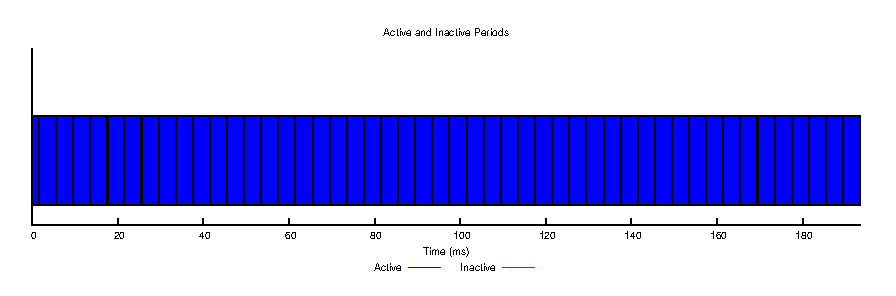
\includegraphics[scale=1]{A1P1.eps}
    \label{fig:plot}
\end{figure}

\newpage

The following is a table with the first 15 samples of the experiment

\begin{figure}[h]
    \caption{Samples}
    \begin{tabular}{c|c|c}
        Sample & Active (ms) & Inactive (ms) \\
        \hline
        1  & 1.502190 & 0.011074 \\
        2  & 3.987884 & 0.003625 \\
        3  & 3.995221 & 0.019725 \\
        4  & 3.979117 & 0.004095 \\
        5  & 3.994876 & 0.011533 \\
        6  & 0.058799 & 0.007539 \\
        7  & 3.920979 & 0.002301 \\
        8  & 3.999042 & 0.138075 \\
        9  & 3.858219 & 0.005810 \\
        10 & 3.995646 & 0.003678 \\
        11 & 3.995211 & 0.001495 \\
        12 & 3.997288 & 0.005308 \\
        13 & 3.993599 & 0.002890 \\
        14 & 3.996001 & 0.001489 \\
        15 & 3.997299 & 0.003389
    \end{tabular}
    \label{fig:samples}
\end{figure}

\subsection{Observations}
From the data we can safely assume that the time slice our single process is receiving before the
timer interrupt fires is 4 milliseconds long. As for the time it takes to service a timer interrupt,
it seems to vary. Perhaps the operating system is performing other maintenance operations during the
interrupt. However, if we exclude some of the outliers like sample 8 in
\hyperref[fig:samples]{\textbf{figure \ref*{fig:samples}}} we come up with an average of $2.4$
microseconds for a timer interrupt using all 50 samples. Refer to the ``format\_data\_A1'' program
for further details on how the average was computed.

It should be noted that it seems like one other non-timer interrupt occurred during data collection.
Referring to sample 6 in \hyperref[fig:samples]{\textbf{figure \ref*{fig:samples}}}, we see that our
process was interrupted shortly after the active period began. Since the data was collected over an
SSH session, this may be an interrupt related to network I/O. However, it could certainly be some
other device.

\subsection{Conclusions}
It appears that our hypothesis is correct. The active process received most of the CPU time during
the experiment and timer interrupts were not expensive at all, taking only $2.4$ microseconds to
service on average. \\

\newpage

\section{Context switching}
\begin{figure}[h]
    \caption{Context switching}
    \centering
    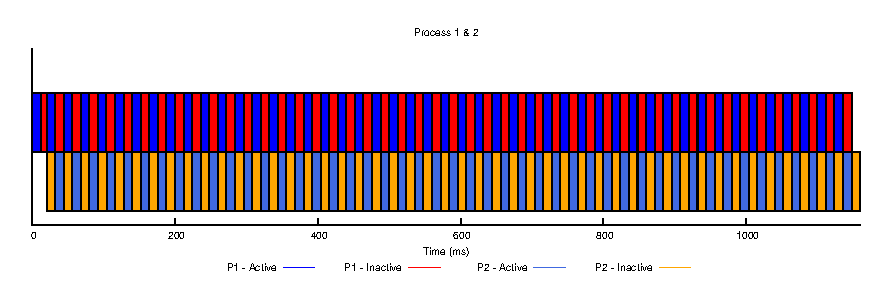
\includegraphics[scale=1]{A1P2.eps}
    \label{fig:plot}
\end{figure}

% ----------------------------------------------------------------
\end{document}
% ----------------------------------------------------------------
